\chapter{Theoretical Background}

In this chapter the theoretical concepts used throughout the report is presented. Knowledge of two computer vision related fields is necessary to understand the following chapters. These are projective geometry, and image processing.

\section{Projective geometry}
Everyone has a basic understanding of what projective geometry is, and how it works.
We experience it at every wake moment, without thinking about it. 
Based on where one is standing and when looking at a shape, the shape can look very different. % TODO ändra
Projective geometry describes these kinds of phenomena.
In this section some basic concepts in projective geometry is presented, and how images are formed in cameras.

At first glance it seems that very little is preserved by a projective transformation, or "changing perspective" in informal term.
Neither shape, lengths, angles, distances, or ratios of distances are preserved.
The most general property in a scene that is preserved by a projective transformation is straightness. \cite[1]{hartley-zisserman}

In euclidean geometry, a point in two-dimensional space is typically represented by cartesian coordinates, a pair of numbers, which represent the distance to the origin in each dimension. % TODO rephrase
In projective geometry homogeneous coordinates are used instead.
To convert the cartesian coordinate pair $(x,y)$ to homogeneous coordinates, a one is appended to the cartesian coordinates, resulting in the point $(x,y,1)$. 
An interesting property about homogeneous coordinates is that they ignore scale, meaning that $(x,y,1)$ and $(kx,ky,k)$ represents the same point for any nonzero value $k$.
To convert back to cartesian coordinates, divide by $k$ and remove the $1$.\cite[2]{hartley-zisserman} % Rephrase this part

\subsection{Camera Model}\label{camera-model}
Cameras, create a 2D representation of a 3D world.
The camera model used in this thesis is called the projective camera model.
It is based on a pinhole camera model, where all rays of light pass through a single point called the camera centre, $C$. Before reaching $C$, each ray will pierce the image plane, where the image is projected.
It's location is determined by $f$, the focal length of the camera.

\begin{figure}
\begin{center}
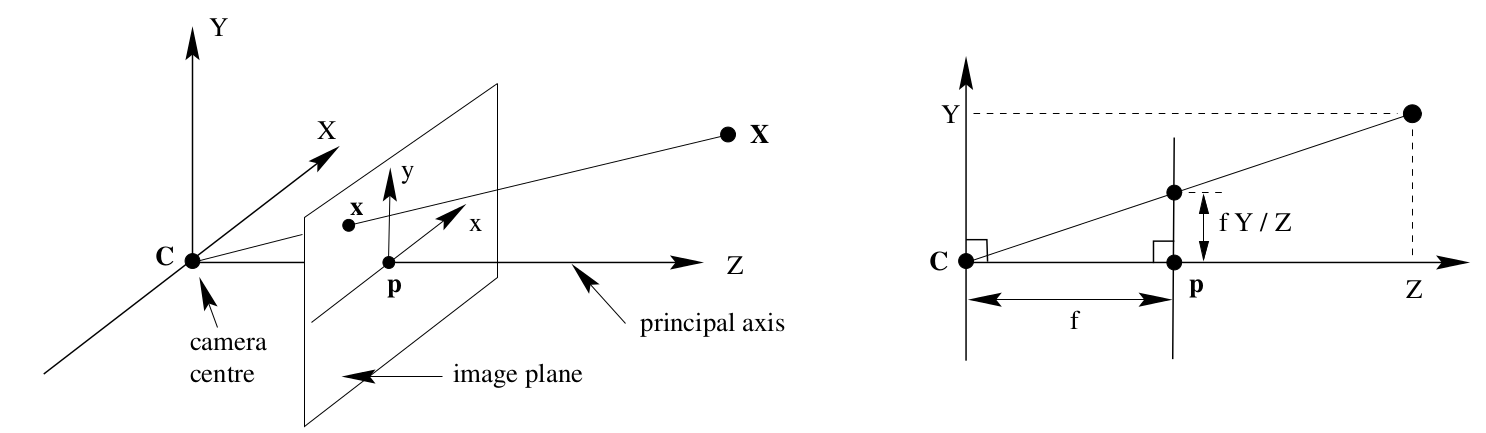
\includegraphics[width=0.6\textwidth]{figures/central_projection_camera.png}
\end{center}
\caption{The central projection camera model. The world and image coordinate systems are aligned. The image plane centred on the $Z$ axis, length $f$ in front of the origin.}
\label{fig:central_projection_camera} % TODO hur referera? zisserman-hartley s.154
\end{figure}

Using the central projection model, as shown in figure \ref{fig:central_projection_camera}, a 3D point can be mapped to a 2D image point, as follows: $(X,Y,Z)^T\mapsto(fX/Z,fY/Z)^T$.
The central projection model makes some rather limiting assumptions, which, which we will now generalise.
First, the origin of the image coordinate system is normally not in the centre.
In that case an offset to the principal point, $(p_{x}, p_{y})$, is added, which represents the coordinates of the centre of the image.
Furthermore, the mapping above assumes that the camera is not rotated, and located in the origin of the world coordinate system. Taking this into account, the following equation can be formed:
\begin{equation}\label{eq:projection1}
\begin{pmatrix}	\tilde{u}\\\tilde{v}\\\tilde{w}\end{pmatrix} = 
\begin{pmatrix}
	f & 0 & p_{x} & 0\\
	0 & f & p_{y} & 0\\
	0 & 0 & 1 & 0
\end{pmatrix}
\begin{pmatrix}
	r_{11} & r_{12} & r_{13} & t_{1}\\
	r_{21} & r_{22} & r_{23} & t_{2}\\
	r_{31} & r_{32} & r_{33} & t_{3}
\end{pmatrix}
\begin{pmatrix}	X\\Y\\Z\\1\end{pmatrix}
\end{equation}

where $(\tilde{x},\tilde{y},\tilde{z})^T$ are the homogeneous coordinates of the pixel in the image of the world coordinates $(X,Y,Z)$.
As explained earlier, the cartesian coordinates are obtained by dividing by $\tilde{w}$:
$$
u = \frac{\tilde{u}}{\tilde{w}},~~v = \frac{\tilde{v}}{\tilde{w}}
$$
The above is the projective camera model that will be used in this thesis. 
It can be generalised further to take things like pixel skew and non-square pixels into account, but those are rare cases and are therefore left out.

The left of the two matrices above is called the calibration matrix, or intrinsic matrix, $K$.
It contains the intrinsic parameters of the camera.
The intrinsic parameters depend only on the camera, and is always the same for the a given camera, if there is no change in zoom.
The right matrix is called the extrinsic matrix, and contains the extrinsic parameters of the camera.
The extrinsic parameters are not tied to the camera's properties, but instead depend on where in the world the camera is located, and where it points.
The above can also be written in the more concise form $x = K[R|t]X$.

When multiplied together, the intrinsic and extrinsic matrices form a $3\times4$-matrix, called the camera matrix, or the projection matrix, $P$:
\begin{equation} \label{eq:projection2}
\begin{pmatrix} \tilde{u} \\ \tilde{v} \\ \tilde{w} \end{pmatrix} = \lambda
\begin{pmatrix} p_{11} & p_{12} & p_{13} & p_{14} \\
 				p_{21} & p_{22} & p_{23} & p_{24} \\
				p_{31} & p_{32} & p_{33} & p_{34} \end{pmatrix}
\begin{pmatrix}X \\Y \\Z \\1\end{pmatrix}
\end{equation}
It can be determined up to an arbitrary scale factor, $\lambda$.
Because $\lambda$ is arbitrary, $P$ only has 11 degrees of freedom. We can simplify to:
\begin{equation}\label{eq:projection3}
\begin{pmatrix} \tilde{u} \\ \tilde{v} \\ \tilde{w} \end{pmatrix} =
\begin{pmatrix} p_{11} & p_{12} & p_{13} & p_{14} \\
 				p_{21} & p_{22} & p_{23} & p_{24} \\
				p_{31} & p_{32} & p_{33} & 1 \end{pmatrix}
\begin{pmatrix}X \\Y \\Z \\1\end{pmatrix}
\end{equation}
where the scaling of the elements of $P$ is implicit for convenience. \cite[153-165]{hartley-zisserman}

\subsection{Planar Homographies}\label{planar-homographies}

\begin{figure}
\begin{center}
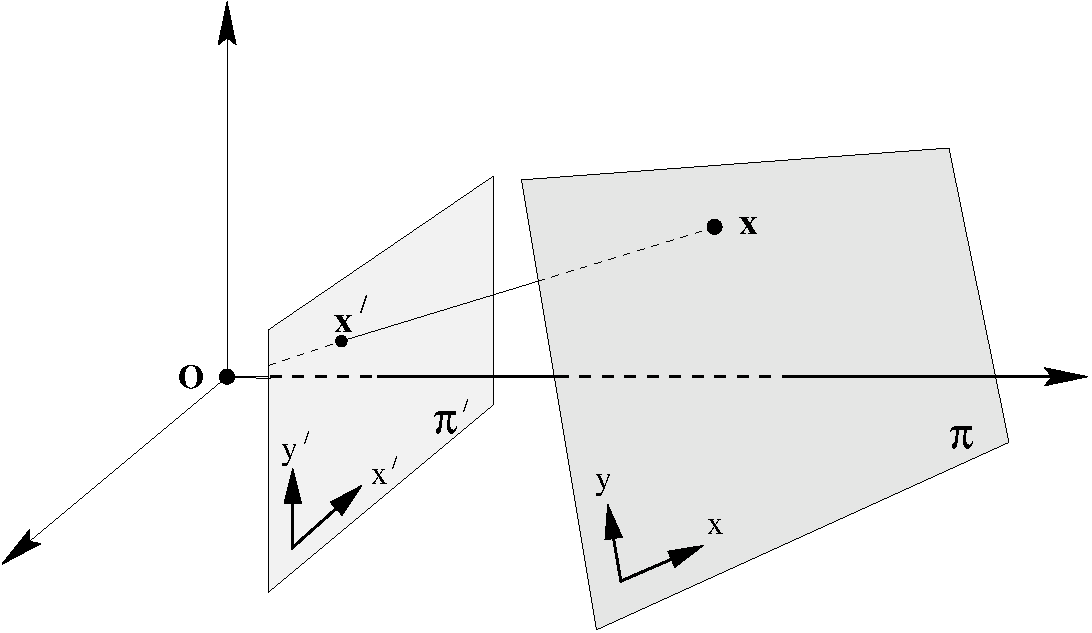
\includegraphics[width=0.6\textwidth]{figures/planar_homography.pdf}
\end{center}
\caption{A point on a plane in the world is projected to the image plane. A planar homography can be used to map points between the two planes} % TODO hur referera? Tagen från hartley-zisserman s. 34
\label{fig:planar_homography}
\end{figure}

Assume that a projective camera is viewing a planar scene, and that we would like to map points on the plane to points on the image plane. 
If the world coordinate system is defined to have its origin in the plane, with the $Z$ axis being perpendicular to it, the projective camera model can be simplified. 
Because $Z=0$ for all coordinates in the plane, the $Z$ coordinate can be removed from the world coordinate vector, along with the third column of the camera matrix, which is cancelled out when $Z=0$. 
This scenario, which is depicted in figure \ref{fig:planar_homography}, yields the following system:
\begin{equation}\label{eq:homography}
\begin{pmatrix} \tilde{u} \\ \tilde{v} \\ \tilde{w} \end{pmatrix} =
\begin{pmatrix} h_{11} & h_{12} & h_{13}  \\
 				h_{21} & h_{22} & h_{23}  \\
				h_{31} & h_{32} & 1\end{pmatrix}
\begin{pmatrix}X \\Y \\ 1\end{pmatrix}
\end{equation}
This transformation is called a planar homography.
The above system is also denoted $x=HX$.

$H$ has 8 degrees of freedom, which means that it can be determined with 8 constraints. Each point correspondence adds 2 constraints on $H$, since each point has 2 degrees of freedom.
Hence, a minimum of 4 point correspondences are required to determine $H$.
In order to uniquely determine $H$, the 8 resulting equations must of course be independent, otherwise the solution is \textit{degenerate}, and does not uniquely determine $H$.
In a minimal solution degeneracy occurs if three of the corresponding points are collinear. \cite[91-92]{hartley-zisserman} % TODO hur citera flera sidor? citera sidor öht?
One method for to determine $H$ from a set of point correspondences is called the Direct Linear Transformation algorithm.
DLT is a simple algorithm which involves forming constraints based on similarity relations (e.g. the point correspondences), and then solving a linear equation system.
Since the positions of the points are often noisy, a more accurate estimate can be achieved if the system is overdetermined, i.e. there are more than four point correspondences.
\cite{homography-estimation}

\subsection{The Plane at Infinity and the Absolute Conic} \label{ac}
Two critical concepts in projective geometry are the plane at infinity, $\pi_{\infty}$ and the absolute conic, $\omega_{\infty}$.
These are very theoretical concepts and will only be touched upon briefly due to their importance for camera calibration.

As mentioned earlier, parallelism is not preserved by projective transformations. % förklarat begreppet projective transformations tidigare?
As a consequence, lines that are parallel in euclidean space are not parallel in projective space, but intersect at a vanishing point, just like parallel train tracks meet at the horizon.

Informally, $\pi_{\infty}$ can be defined as a plane in projective space where parallel lines meet. 
On the $\pi_{\infty}$ lies the imaginary, absolute conic, $\omega_{\infty}$.
Its projection onto the image plane is called the Image of the Absolute Conic.
The full theory regarding these concepts is out of scope for this thesis, but the important thing to know is that $\omega_{\infty}$ is invariant to projective transformations.
This has important implications for camera calibration because, because it means that $\omega_{\infty}$ acts as a natural calibration object present in every image.
It can be shown that the following relationship exists between $K$ and the image of the image of the absolute conic:
$\omega = (KK^T)^{-1}$. \cite[210]{hartley-zisserman}\cite{pollefeys}

\subsection{Camera Calibration} \label{camera-calibration}
This section will describe how to determine the camera matrix $P$, and its components.
This problem is known as camera calibration, or camera resectioning.
It is a very similar problem to the one described in \ref{planar-homographies}, and can be solved in the same manner.	
The calibration matrix $K$ can then be extracted from $P$, using QR-decomposition.\cite{wiki:qr-decomposition}
$K$ can then be reused to determine the camera pose, even when observing a different scene, as described in \ref{camera-pose}.

The different from the 2D case is that matrix has an extra column. The number of unknowns is now eleven instead of eight, which means that five and a half point correspondences (meaning five points and one $x$ or $y$ correspondence) are needed instead of four.
The problem of degeneracy is also more complicated than in the 2D case.
The most important case is that degeneracy occurs if all points lie in the union of a plane and a line. \cite[179-180]{hartley-zisserman}

A classic strategy for calibrating cameras is to use orthogonal planes with a known pattern on them. 
Since the planes are orthogonal, degeneracy can be avoided.

A simpler, and widely used approach was presented by Zhengyou Zhang in his paper "Flexible Camera Calibration By Viewing a Plane From Unknown Orientations".
Zhang's method uses multiple images (at least two) from different perspectives of a single known, planar pattern.
If many images are known the chance of degeneracy is low, and  the solution becomes very over-determined, which helps improve accuracy.
Furthermore this method considers radial distortion in the lens, which can be used to further improve accuracy. \cite{zhang-calibration}

\subsubsection{Camera calibration using Vanishing Points}
Another approach to calculate $K$ is to do so without first calculating $P$, by using vanishing points.
It turns out that $K$ can be determined from a single image, by imposing constraints on the image of the absolute conic ($\omega$) and then using the equation presented in \ref{ac} to find $K$.

Like $K$, $\omega$ is represented by a symmetric, homogeneous matrix with the following structure
$$
\omega = \begin{pmatrix}
	w_{1} & w_{2} & w_{4} \\
	w_{2} & w_{3} & w_{5} \\
	w_{4} & w_{5} & w_{6} 
\end{pmatrix}
$$
which can be derived the fact that the structure of $K$ is known, and $\omega = (KK^T)^{-1}$.

There are three types of constraints that can be imposed on $\omega$:
\begin{enumerate}
	\item metric information from a plane in the image with a known homography
	\item information from orthogonal vanishing points
	\item internal constraints from $K$, like no skew or square pixels.
\end{enumerate}

We will begin with the latter type.
If it is known that pixels are square, as is assumed in this thesis, then $\omega$ has the following form:
$$
\omega = \begin{pmatrix}
	w_{1} & 0 & w_{2} \\
	0 & w_{1} & w_{3} \\
	w_{2} & w_{3} & w_{4}
\end{pmatrix}
$$
Now, only three constraints are needed (because $\omega$ is homogeneous).

Orthogonal vanishing points give rise to constraints of the form $V_{1}^T \omega v_{2} = 0$.
A known homography $H=[h_{1},h_{2},h_{3}]$ give the two constraints $h_{1}^T \omega h_{2} = 0$ and $h_{1}^T \omega h_{1} = h_{2}^T \omega h_{2}$. Refer to \cite{hartley-zisserman} chapter 8 to see how they are derived.

Each constraint can be rewritten to the form $aw=0$ where $a$ is a $1 \times 4$ vector representing the constraint, and $w$ is the vector $w = (w_1,w_2,w_3,w_4)$ containing the elements of $\omega$.
The $n$ constraint vectors are then stacked on top of each other which leads to the system $Aw=0$ where $A$ is a $n \times 4$ matrix and $0$ is a $4 \times 1$ zero vector. % TODO proper vector notation
This system can be solved using SVD to determine $\omega$.
Finally, $\omega$ is decomposed into $K$ by matrix inversion followed by Cholesky factorization.\cite[223-226]{hartley-zisserman}

\subsubsection{Obtaining Camera Pose with known $K$} \label{camera-pose}
When $K$ is known, the final step before points can be projected using equation \ref{eq:projection1}, is to determine the pose of the camera, i.e. the matrix $[R|t]$. $R|t]$ reprents the rotation and translation of the camera in the world coordinate frame, where $R$ is a $3 \times 3$ matrix and $t$ is a $3 \times 1$ vector.
Constraints can be imposed through point correspondences like in previous cases.
The $R$ and $t$ have three degrees of freedom each, which means six constraints are required to determine them.
As a result, three point correspondences are required to determine the pose, since each correspondence generates two constraints.
But since the resulting system is non-linear in this case, so DLT cannot be used here. \cite[187]{hartley-zisserman}
However, there exist a large number of techniques to solve this problem which is known as Perspective-n-Point (PnP).
Both iterative, e.g. \cite{hesch-pnp} \cite{oberkampf-pnp}, and non-iterative solutions exist, e.g. \cite{quan-pnp} \cite{lepetit-pnp}.
The latter method is called EPnP.
It is presented in a fairly recent paper, and claims to be both faster and more accurate than other methods. 

\section{Image Processing}
Image processing concerns processing of digital images, which consist of small image elements, pixels.
A distinction is often made between the field of image processing and image analysis, where image processing refers to low-level processing, and image analysis concerns high-level processing.
Both the input and output of an image processing algorithm are typically images, for example algorithms for noise, contrast enhancement, and colour correction. 
In contrast, the input of an image analysis algorithm is typically an iamge, but the output is some representation of features in the image.
The task could example be image segmentation, i.e. the task of dividing an image into regions or objects.\cite[p. 1-2]{pitas}\cite[p. 1-2]{gonzalez-woods}
In this thesis the two concepts will be used interchangeably henceforth.
TODO What to write? How detailed?% TODO write

















